\documentclass[a4paper, 12pt, oneside]{scrbook}

\usepackage[ngerman]{babel}		
\usepackage[onehalfspacing]{setspace}  %Zeilenabstand 1.5
\PassOptionsToPackage{hyphens}{url}\usepackage[hidelinks]{hyperref}

\usepackage[backend=biber,style=numeric,sorting=none]{biblatex}
\usepackage[T1]{fontenc}	  	
\usepackage[utf8]{inputenc}
\usepackage{acronym}
\usepackage[left=2.5cm,right=2.5cm,top=2.5cm,bottom=2.5cm,includeheadfoot]{geometry} % 2.5cm Randabstand werden als Minimum von der DHBW vorgeschrieben
\usepackage{graphicx}
\usepackage{epstopdf}
\usepackage{float}
\usepackage{booktabs}
\usepackage{caption}
\usepackage{csquotes}
\usepackage{fancyhdr}
\usepackage{wrapfig}
\usepackage{scrhack}

\usepackage{blindtext}
\usepackage[parfill]{parskip} % Entfernt Einrückung zu Beginn eines Paragraphen

\renewcommand*{\headfont}{\normalfont}
\renewcommand*{\multicitedelim}{\addsemicolon\space}
\renewcommand*{\headrulewidth}{0pt}
\renewcommand*{\arraystretch}{1.5}

\setlength{\parskip}{1.5ex}

\usepackage{comment}

% Code Formatierung
\usepackage{listings}
\usepackage{color}

\renewcommand{\lstlistingname}{Codebeispiel}
\renewcommand{\lstlistlistingname}{Codebeispielverzeichnis}

\definecolor{dkgreen}{rgb}{0,0.6,0}
\definecolor{gray}{rgb}{0.5,0.5,0.5}
\definecolor{mauve}{rgb}{0.58,0,0.82}

\lstset{frame=tb,
	language=Java,
	morekeywords={typeof, new, true, false, catch, function, return, null, catch, switch, var, if, in, while, do, else, case, break},
	ndkeywords={class, export, boolean, throw, implements, import, this, await, async},
	aboveskip=3mm,
	belowskip=3mm,
	showstringspaces=false,
	columns=flexible,
	basicstyle={\small\ttfamily},
	numbers=none,
	numberstyle=\tiny\color{gray},
	keywordstyle=\color{blue},
	commentstyle=\color{dkgreen},
	stringstyle=\color{mauve},
	breaklines=true,
	tabsize=3,
	captionpos=b
}

\bibliography{bibliography.bib}
\begin{document}

\frontmatter

% Hierin müssen Matrikelnummer Name usw. gesetzt werden.
\def\doctype{Dokumententyp}
\def\title{Entwicklung einer Webanwendung unter Verwendung des Angular-Frameworks, welche die Verwaltung von Schichtwechsel für Mitarbeiter unterstützt}
\def\author{Lars Rickert}

\begin{titlepage}

	\vspace{10mm}

	\begin{center}
		\vspace{5mm}

		\huge \title

		\vspace{14.2pt}

		%\large \doctype


		\vspace{42.6pt}

		\large Studienarbeit T3\_3101

		\vspace{42.6pt}

		\small des Studienganges Angewandte Informatik an der \\
		\large Dualen Hochschule Baden-Württemberg Mosbach

		\vspace{14.2pt}

		
\includegraphics[height=1.5cm]{prefix/image/logo-dhbw.pdf}

		\vspace{42.6pt}

		\small von \\
		\large \author
	\end{center}

	\vspace{140pt}

	\begin{table}[h]
		\centering
		\begin{tabular}{ll}
			% \small Bearbeitungszeitraum            & XXX Wochen     \\
			\small Matrikelnummer, Kurs            & 4753795, INF21B \\
			\small Gutachter der Dualen Hochschule & Philipp Abele   \\
		\end{tabular}
	\end{table}

	\vspace{49.7pt}

	\fancypagestyle{empty}{
		\fancyhf{}
		\fancyfoot[C]{\today}
	}

\end{titlepage}

\pagenumbering{gobble}
\input{prefix/eigenstaendigkeit.tex}

\tableofcontents

% Abbildungsverzeichnis
\cleardoublepage
\phantomsection
\addcontentsline{toc}{chapter}{\listfigurename}
\pagenumbering{Roman}
\listoffigures

% Tabellenverzeichnis
% \cleardoublepage
% \phantomsection
% \addcontentsline{toc}{chapter}{\listtablename}
% \listoftables

%Codebeispiel Verzeichnis
% \cleardoublepage
% \phantomsection
% \addcontentsline{toc}{chapter}{\lstlistlistingname}
% \lstlistoflistings

% Abkürzungsverzeichnis (siehe Ordner "content")
\chapter{Abkürzungsverzeichnis}
\begin{acronym}
	\acro{VS Code}{Visual Studio Code}
\end{acronym}

\mainmatter

%%%%%% Inhalt (siehe Ordner "content") %%%%%%
\chapter{Einleitung}

In der modernen Arbeitswelt spielen flexible Arbeitszeitmodelle eine zunehmend wichtiger werdende Rolle, um den vielfältigen Anforderungen sowohl der Arbeitgeber als auch der Arbeitnehmer gerecht zu werden. 
Laut einer Studie der International Labour Organization wird Flexibilität in der Arbeitszeitgestaltung als entscheidender Faktor für die Vereinbarkeit von Beruf und Privatleben angesehen und kann die Zufriedenheit und Produktivität der Mitarbeiter signifikant erhöhen \cite[S.12 ff.]{ilo2018}. 
Ein zentrales Element dieser Flexibilität ist die Möglichkeit für Mitarbeiter, Schichten untereinander zu tauschen. 
Oft werden Schichttauschvereinbarungen privat organisiert, beispielsweise über Messenger-Dienste wie WhatsApp. 
%Problemstellung
In vielen Unternehmen organisieren Mitarbeiter ihre Schichtwechsel eigenständig und informell, oft über Messaging-Dienste wie WhatsApp. Dies gilt auch für die Mitarbeiter dieser Firma, die ihre Schichtwechsel in einer WhatsApp-Gruppe privat koordinieren. Ein typisches Beispiel einer solchen Liste für den Monat Januar sieht wie folgt aus:

\begin{figure}[h]
    \centering
    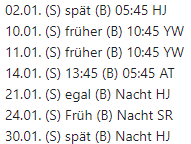
\includegraphics[clip,width=0.25\linewidth]{images/WhatsAppListe.png}
    \caption[Beispiel der Schichtwechsel-Liste aus WhatsApp für Januar]{Beispiel der Schichtwechsel-Liste aus WhatsApp für Januar}
    \label{WhatsAppListe}
\end{figure}

Hierbei steht (S) für "Suche" und (B) für "Biete", gefolgt von den jeweiligen Schichtzeiten und den Initialen der Personen.

Diese manuelle Methode bringt mehrere Herausforderungen und Ineffizienzen mit sich. Die fortlaufende Aktualisierung der Liste in WhatsApp führt oft zu einer unübersichtlichen Flut an Informationen, bei der Änderungen oder neue Einträge leicht übersehen werden können. 
Außerdem erfordert die aktuelle Methode von den Mitarbeitern, die gesamte Kommunikation und Liste in WhatsApp ständig zu überwachen, was zeitaufwendig und unpraktisch ist. Diese Herausforderungen beeinträchtigen die Effizienz der Schichtorganisation und führen zu mehr Unzufriedenheit bei den Mitarbeitern.

Das Ziel dieser wissenschaftlichen Arbeit ist es, ein benutzerfreundliches und effizientes UX Design Konzept zur Organisation von Schichtwechseln zu entwickeln. Dieses Konzept soll die aktuellen Probleme der ineffizienten WhatsApp-basierten Methode adressieren und eine strukturierte, leicht zugängliche und übersichtliche Alternative bieten.
\chapter{Grundlagen}

\section{Google Design Sprint}

Der Google Design Sprint \ac{GDS} ist eine von Jake Knapp bei Google Ventures entwickelte Methodik zur schnellen und effizienten Problemlösung sowie Produktentwicklung, insbesondere für Herausforderungen, die sich aus der dynamischen Natur des Marktes und den sich verändernden Produktanforderungen ergeben. 
Ziel dieser Methode ist es, innerhalb eines Zeitraums von fünf Tagen einen Prototyp zu entwickeln und zu evaluieren. 
Diese Methode bietet den Vorteil, dass nicht auf die Markteinführung gewartet werden muss, um Feedback zu erhalten. Stattdessen können dringende Fragen sofort beantwortet werden \cite[S.98 f.]{Design_Sprint}.

Die fünftägige Methode, wie in Abbildung \ref{GDS} dargestellt, verläuft wie folgt:

\begin{figure}[h]
    \centering
    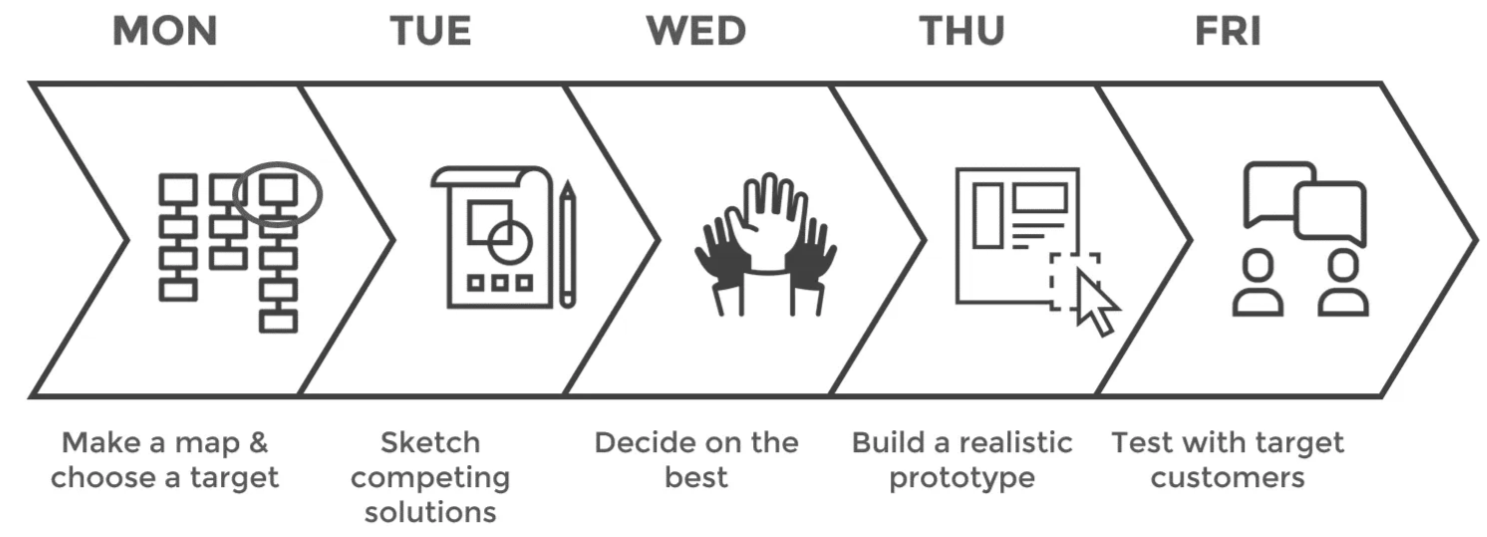
\includegraphics[clip,width=0.75\linewidth]{images/GDS.png}
    \caption[Ablauf eines GDS]{Ablauf eines GDS \cite{GDS_Abbildung}}
    \label{GDS}
\end{figure}

Am ersten Tag geht es darum, das Problem zu verstehen und den Fokus für die Woche festzulegen. Das Team definiert das langfristige Ziel und identifiziert die Herausforderung. 

Am zweiten Tag konzentriert sich das Team auf die Bewältigung bereits bekannter Herausforderungen. Anders als bei herkömmlichen Brainstorming-Sitzungen arbeiten die Teammitglieder einzeln an Lösungsansätzen und folgen einem strukturierten vierstufigen Prozess, um das kritische Denken zu fördern. 

Am dritten Tag trifft das Team Entscheidungen darüber, welche Idee als Prototyp entwickelt und getestet werden sollen. Dabei kommt die fünfstufige "Sticky Decision"-Methode zum Einsatz, um die besten Lösungen zu identifizieren. Anschließend wird ein detaillierter Prozessplan für den Prototypen erstellt. 

Am vierten Tag wird ein realitätsnaher Prototyp entwickelt. Das Ziel ist es, eine testbare Version der Lösung zu erstellen, die am nächsten Tag mit echten Nutzern evaluiert werden kann. 

Der letzte Tag ist für das Testen des Prototyps reserviert. Das Team sammelt Feedback von echten Nutzern und erhält Einsicht, ob die Lösung in der Praxis funktioniert und welche Anpassungen nötig sind. Dieses Feedback ist entscheidend, um die Stärken und Schwächen der entwickelten Lösung zu identifizieren \cite[S.22 ff.]{Design_Sprint}.

\section{User Experience}
Das Design der User Experience \ac{UX} konzentriert sich auf jedes Element und jede Funktion, die der Benutzer bei einer Anwendung sieht, mit dem Ziel, eine möglichst angenehme und effiziente Erfahrung zu ermöglichen \cite[S.12]{Bordegoni}. 
Laut der International Organization for Standardization (ISO 9241-210) wird UX definiert als „Wahrnehmungen und Reaktionen einer Person, die sich aus der Verwendung und/oder der erwarteten Verwendung eines Produkts, Systems oder einer Dienstleistung ergeben” \cite{iso}. 
Während sich das User Interface auf das Erscheinungsbild der Anwendung konzentriert, beispielsweise auf Schriftarten und Farben, geht die UX tiefer und umfasst das gesamte Erlebnis des Nutzers \cite[S.8]{Canziba}.

In den letzten Jahrzehnten hat die Bedeutung der User Experience stark zugenommen, da Unternehmen erkannt haben, dass ein positives Nutzungserlebnis entscheidend für den Erfolg eines Produkts ist \cite{ux_article}. 
Bei einem schlechten UX-Design fällt es den Benutzern schwer, die Anwendung zu nutzen, und sie wechseln, sobald sie eine ähnliche, bessere App gefunden haben, die die gleiche Aufgabe erfüllt. 
Deshalb ist es für ein gutes UX-Design wichtig, dass der Designer die Bedürfnisse der Benutzer vorhersieht und erfüllt, indem er ihre Sichtweise einnimmt. Ein gutes UX-Design kann die Produktivität steigern, die Zufriedenheit der Kunden erhöhen und die Verkaufszahlen verbessern. 
Zudem können durch eine optimierte Benutzererfahrung die Kosten für Support und Wartung gesenkt werden \cite[S.8 ff.]{Canziba}.

Die UX umfasst verschiedene Komponenten, die zusammenarbeiten, um ein positives Nutzungserlebnis zu schaffen. Dazu gehören Usability, Ästhetik, Interaktion und Emotionalität.

Die Usability bezieht sich auf die Benutzerfreundlichkeit und Effizienz eines Produkts. 
Ein System mit hoher Usability ermöglicht es den Nutzern, ihre Ziele schnell und ohne Frustration zu erreichen. 
Dies beinhaltet Aspekte wie Lernfähigkeit, Effizienz der Nutzung und Zufriedenheit der Nutzer \cite[S.23 ff.]{Nielsen}.

Die Ästhetik bezieht sich auf das Erscheinungsbild des Produkts. 
Ein ansprechendes visuelles Design kann die Wahrnehmung der Qualität und den Gesamteindruck eines Produkts erheblich verbessern. 
Studien zeigen, dass ästhetisch ansprechende Designs oft als funktionaler und benutzerfreundlicher wahrgenommen werden \cite{Tractinsky}.
\chapter{Entwicklung der User Experience mit Verwendung des Google Design Sprints}

Die Entwicklung eines nutzerfreundlichen und effektiven UX-Design-Konzepts zur Abstimmung von Schichtwechseln wurde mithilfe des GDS realisiert. Ursprünglich wurde der GDS für einen Zeitraum von fünf Tagen entwickelt, um schnell Lösungen für komplexe Probleme zu finden und neue Ideen zu testen. In diesem Projekt wurde der GDS aufgrund der Durchführung durch eine Einzelperson angepasst.

Die Phasen 4 und 5 des GDS, die normalerweise die Entwicklung eines Prototypen und das Testen umfassen, wurden modifiziert. Stattdessen wurde ein umfangreiches Bedienungskonzept entwickelt, auf dessen Grundlage eine Nutzerumfrage durchgeführt wurde (siehe Kapitel~\ref{chap:nutzerumfrage}) .
Die Ergebnisse dieser Umfrage wurden anschließend genutzt, um den Prototypen zu erstellen.
%(siehe Kapitel~\ref{chap:prototyp}) 

\section{Phase 1: Verstehen und Definieren}
In der ersten Phase werden die benötigten Informationen gesammelt und analysiert, um das Problem umfassend zu verstehen und klar zu definieren. Die Problemstellung und Zielsetzung wurden bereits in der Einleitung ausführlich behandelt, daher wird in diesem Kapitel direkt auf die praktische Anwendung der nächsten Phasen eingegangen.

\section{Phase 2 und 3: Skizzieren und Auswahl der Idee}
In der Skizzieren Phase beginnt der Prozess der Designerstellung. Hierbei wurden sich zunächst die benötigten Seiten überlegt, um die benötigten Aufgaben und Anforderungen zu erfüllen. Dazu gehört eine Übersichtsseite auf der alle aktuellen Tauschangebote stehen und worüber der Nutzer zu allen weiteren Seiten gelangt, z.B. die zum Hinzufügen und zum Annehmen eines Tauschangebots, sowie eine Seite, auf der der Nutzer seine angenommen Schichten sehen kann und individuelle Einstellungen vornehmen kann. 

Die erste Version der Übersichtsseite war zunächst für einen Desktop ausgelegt (siehe Abbildung \ref{Version1_Desktop}). 

\begin{figure}[h]
    \centering
    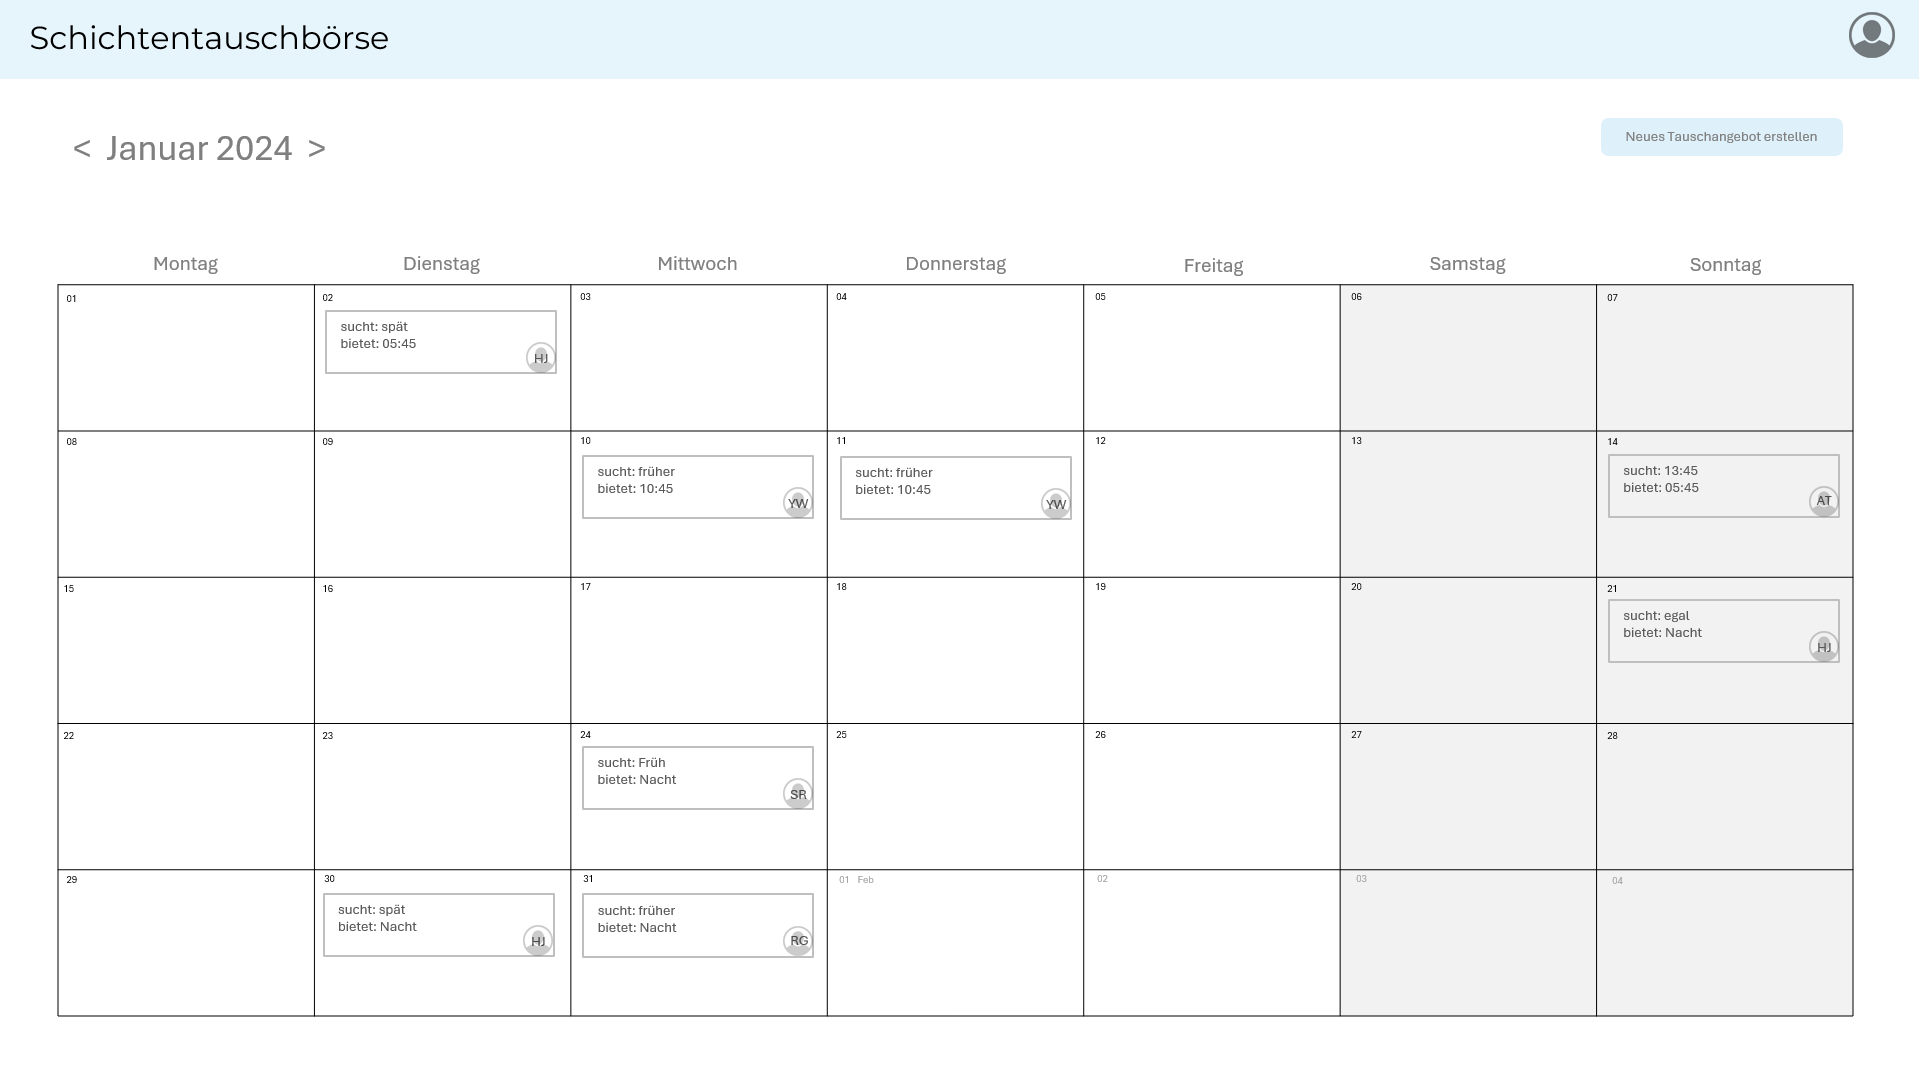
\includegraphics[clip,width=0.9\linewidth]{images/Version1_Desktop.png}
    \caption[Erste Version der Übersichtsseite für den Desktop]{Erste Version der Übersichtsseite für den Desktop}
    \label{Version1_Desktop}
\end{figure}

Im oberen Bereich der Seite befindet sich der Header. 
Links darunter hat der Nutzer die Möglichkeit zwischen den Monaten zu navigieren. 
Rechts unter dem Header befindet sich “Neues Tauschangebot erstellen” Button, mit dem Nutzer neue Tauschangebote erstellen können. 
Zentral auf der Seite ist der Kalender des aktuellen Monats groß dargestellt, die Wochentage sind darüber ausgeschrieben.

Bei der Übertragung des Designs in die Handy-Version wurden einige Schwachstellen identifiziert. Die Darstellung des Desktop-Designs auf dem Handy führt dazu, dass die Schrift aufgrund der kleinen Größe schlecht lesbar war (siehe Abbildung \ref{Version12_Handy}). 

\begin{figure}[h]
    \centering
    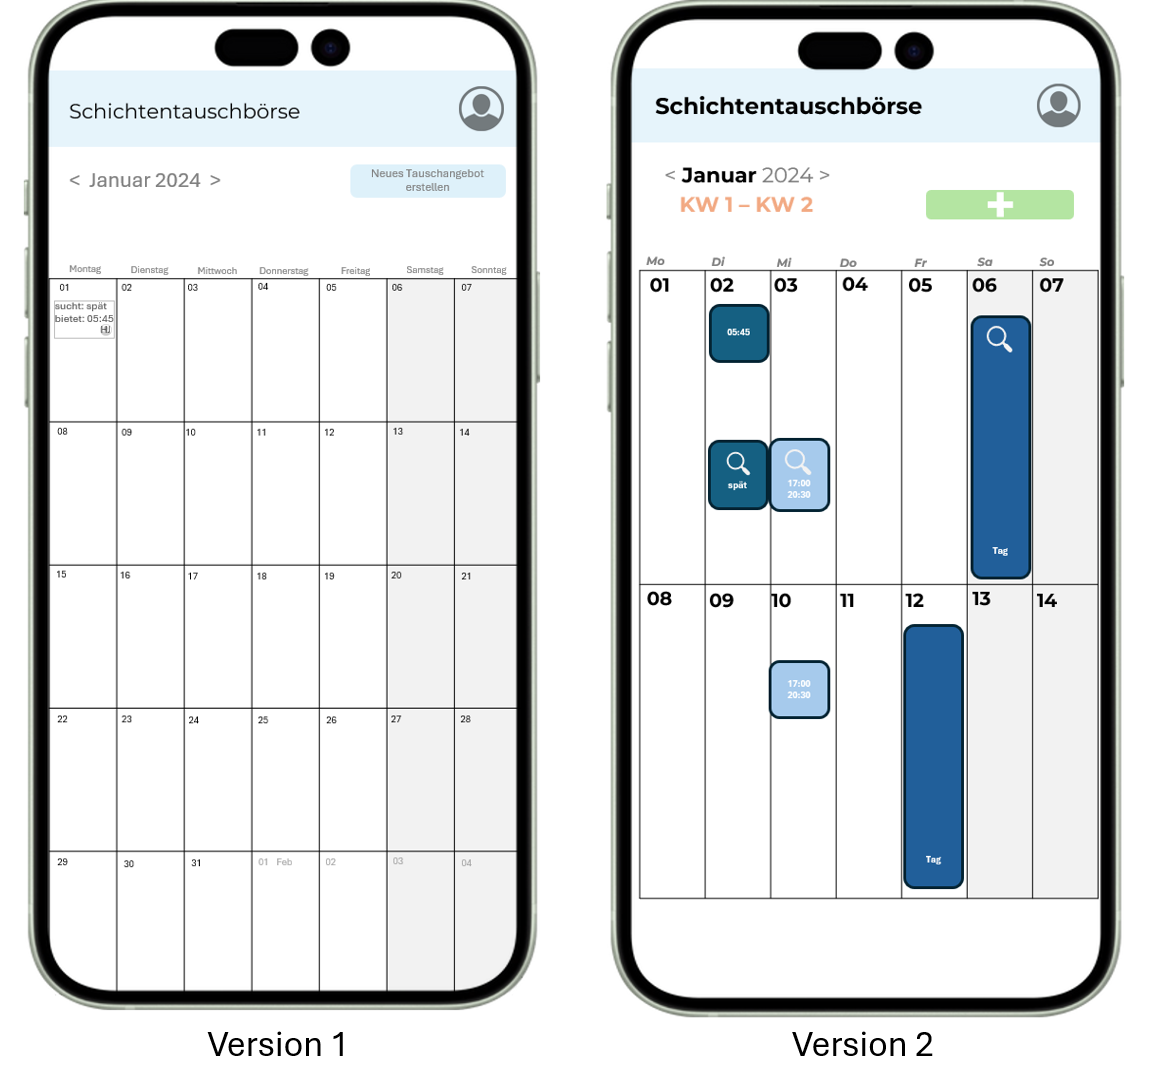
\includegraphics[clip,width=0.75\linewidth]{images/Version12_Handy.png}
    \caption[Erste und zweite Version der Übersichtsseite für das Handy]{Erste und zweite Version der Übersichtsseite für das Handy}
    \label{Version12_Handy}
\end{figure}

Da die meisten Nutzer die App wahrscheinlich auf dem Handy verwenden möchten, wurde das Design in Version 2 entsprechend angepasst.

Um in der Kalenderübersicht die Tauschanfragen gut lesbar und nutzerfreundlich darzustellen, werden statt fünf Wochen nur noch zwei Wochen angezeigt (siehe Version 2 in Abbildung \ref{Version12_Handy}). 
Aufgrund der schmaleren Handybildschirme wird ein Teil der Wörter durch Piktogramme ersetzt, z.B. wurde beim “Neues Tauschangebot erstellen” Button der Text durch ein Plus ersetzt. Dadurch wird Platz gespart und die Funktion wird klarer erkannt. 
Außerdem werden die Wochentage nicht mehr ausgeschrieben. Eine weitere Änderung ist, dass die Schichten in den gesuchten/gebotenen Zeit Blöcken am Tag abgebildet (siehe Version 2 in Abbildung \ref{Version12_Handy}).

Allerdings wurde festgestellt, dass der Kalender unübersichtlich wird, wenn mehrere Tauschangebote an einem Tag sind oder wenn welche zum gleichen Zeitpunkt angefragt werden. 
Deswegen wird eine weitere Version erstellt, in der die Schichten nicht mehr nach dem Zeitpunkt sortiert sind, sondern in einem Block organisiert, was eine bessere Übersicht ermöglicht (siehe Abbildung \ref{Version3_Handy}).

\begin{figure}[h]
    \centering
    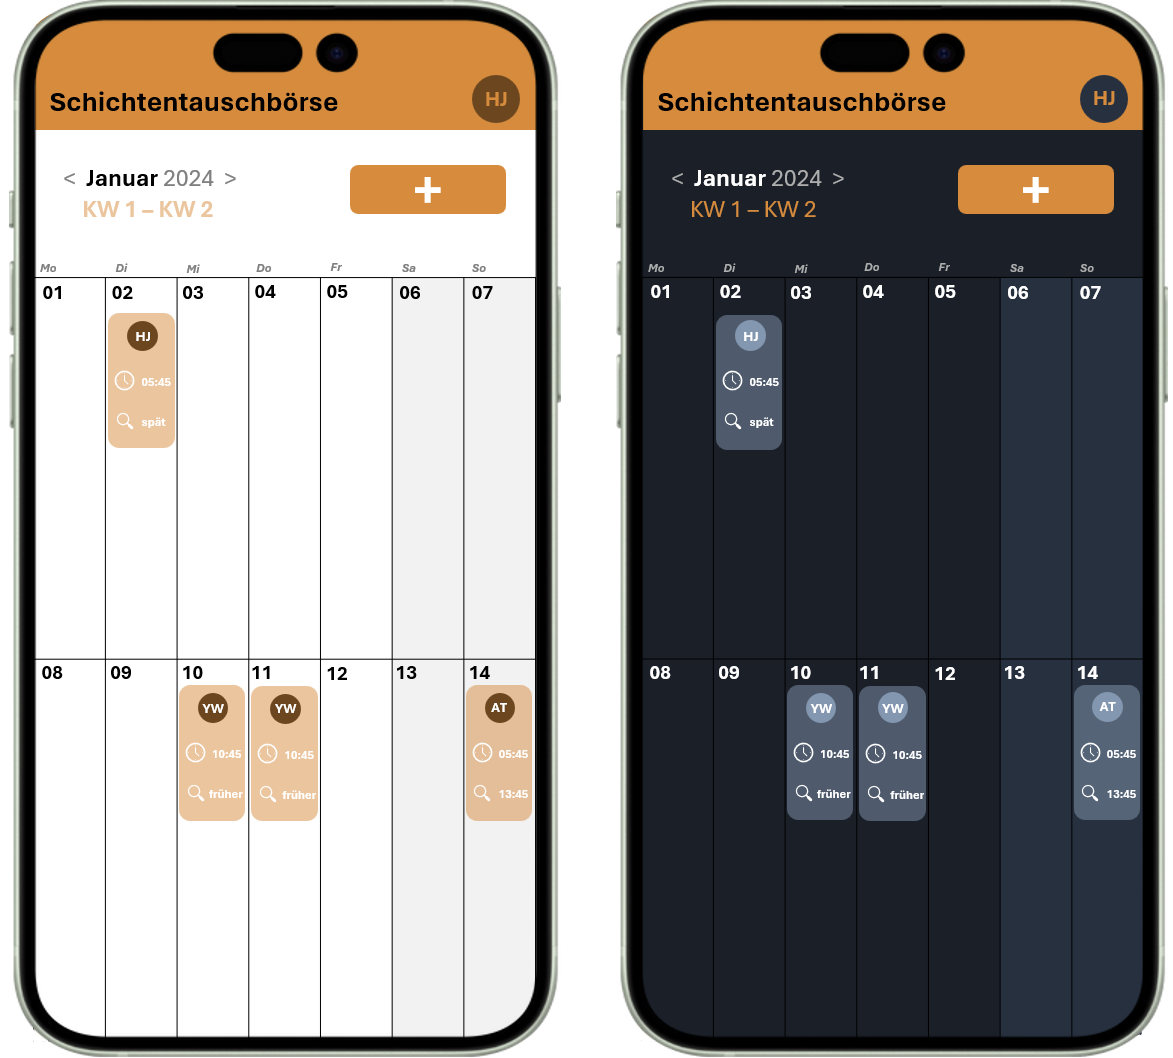
\includegraphics[clip,width=0.75\linewidth]{images/Version3_Handy.png}
    \caption[Dritte Version der Übersichtsseite für das Handy, im Light Mode und Dark Mode]{Dritte Version der Übersichtsseite für das Handy, im Light Mode und Dark Mode}
    \label{Version3_Handy}
\end{figure}

Des weiteren wurde die Hauptfarbe von einem hellen Blau zu einem Orange gewechselt, welches wärmer und aktiver wirkt. Da der Dark Mode in den letzten Jahren stark an Popularität zugenommen hat \cite{diva2020darkmode} wird für die Anwendung auch ein Farbkonzept erstellt (siehe Dark Mode in Abbildung \ref{Version3_Handy}). 

Für die dritte Version wurde sich letztendlich entschieden. Darauf aufbauend wurden die weiteren Seiten der Anwendung im Light Mode gestaltet.

\section{Phase 4: Entwicklung des Bedienungskonzepts}
\label{sec:bedienungskonzept}
Um den Nutzern eine bessere Vorstellung von der UX zu vermitteln, wurden zwei unterschiedliche Farbpaletten erstellt: eine für den Light Mode und eine für den Dark Mode (siehe Abbildung \ref{Farbpalette}).

\begin{figure}[h]
    \centering
    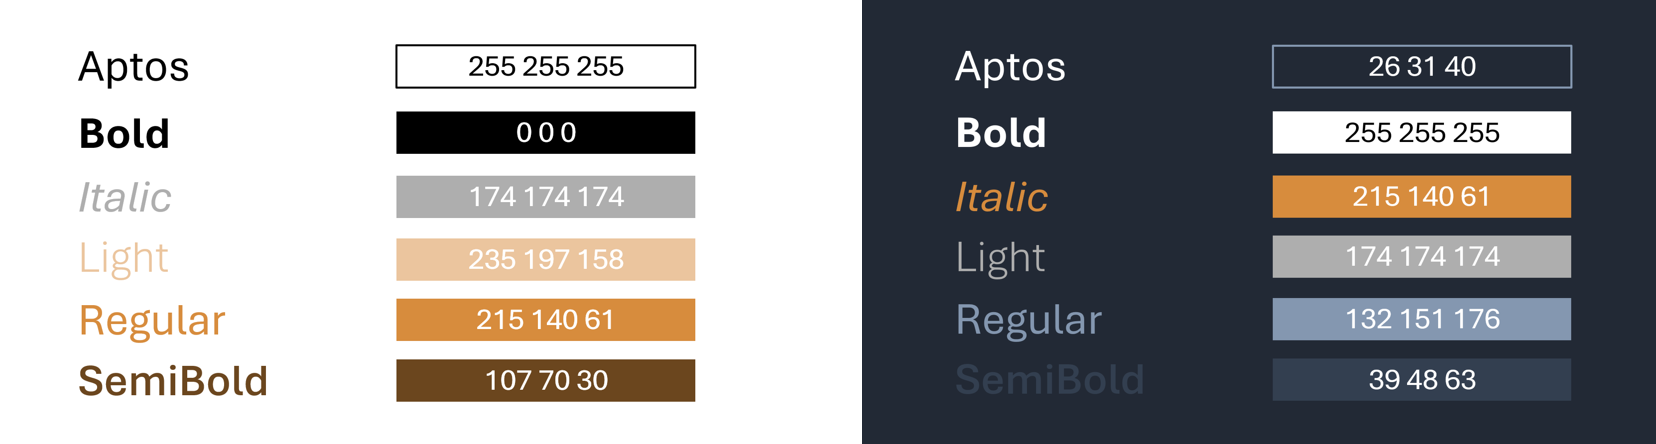
\includegraphics[clip,width=0.9\linewidth]{images/Farbpalette.png}
    \caption[Farbpalette für den Light Mode und Dark Mode]{Farbpalette für den Light Mode und Dark Mode}
    \label{Farbpalette}
\end{figure}

Die Farbpalette für den Light Mode besteht aus verschiedenen Orangetönen und einem Braun. Die Hintergrundfarbe des Dark Modes ist ein dunkles Blau, Orange wird nur noch als Akzentfarbe verwendet, ansonsten wird ein helleres Blau genutzt.
Die Schriftart "Aptos" wurde aufgrund ihrer Lesbarkeit und Ästhetik ausgewählt.

Ein zentrales Element des UX Designs war die Entwicklung eines klaren und intuitiven Bedienungskonzepts. Ziel war es, eine benutzerfreundliche Navigation zu schaffen, die es den Nutzern ermöglicht, alle Funktionen der Anwendung schnell und einfach zu erreichen.

\begin{figure}[h]
    \centering
    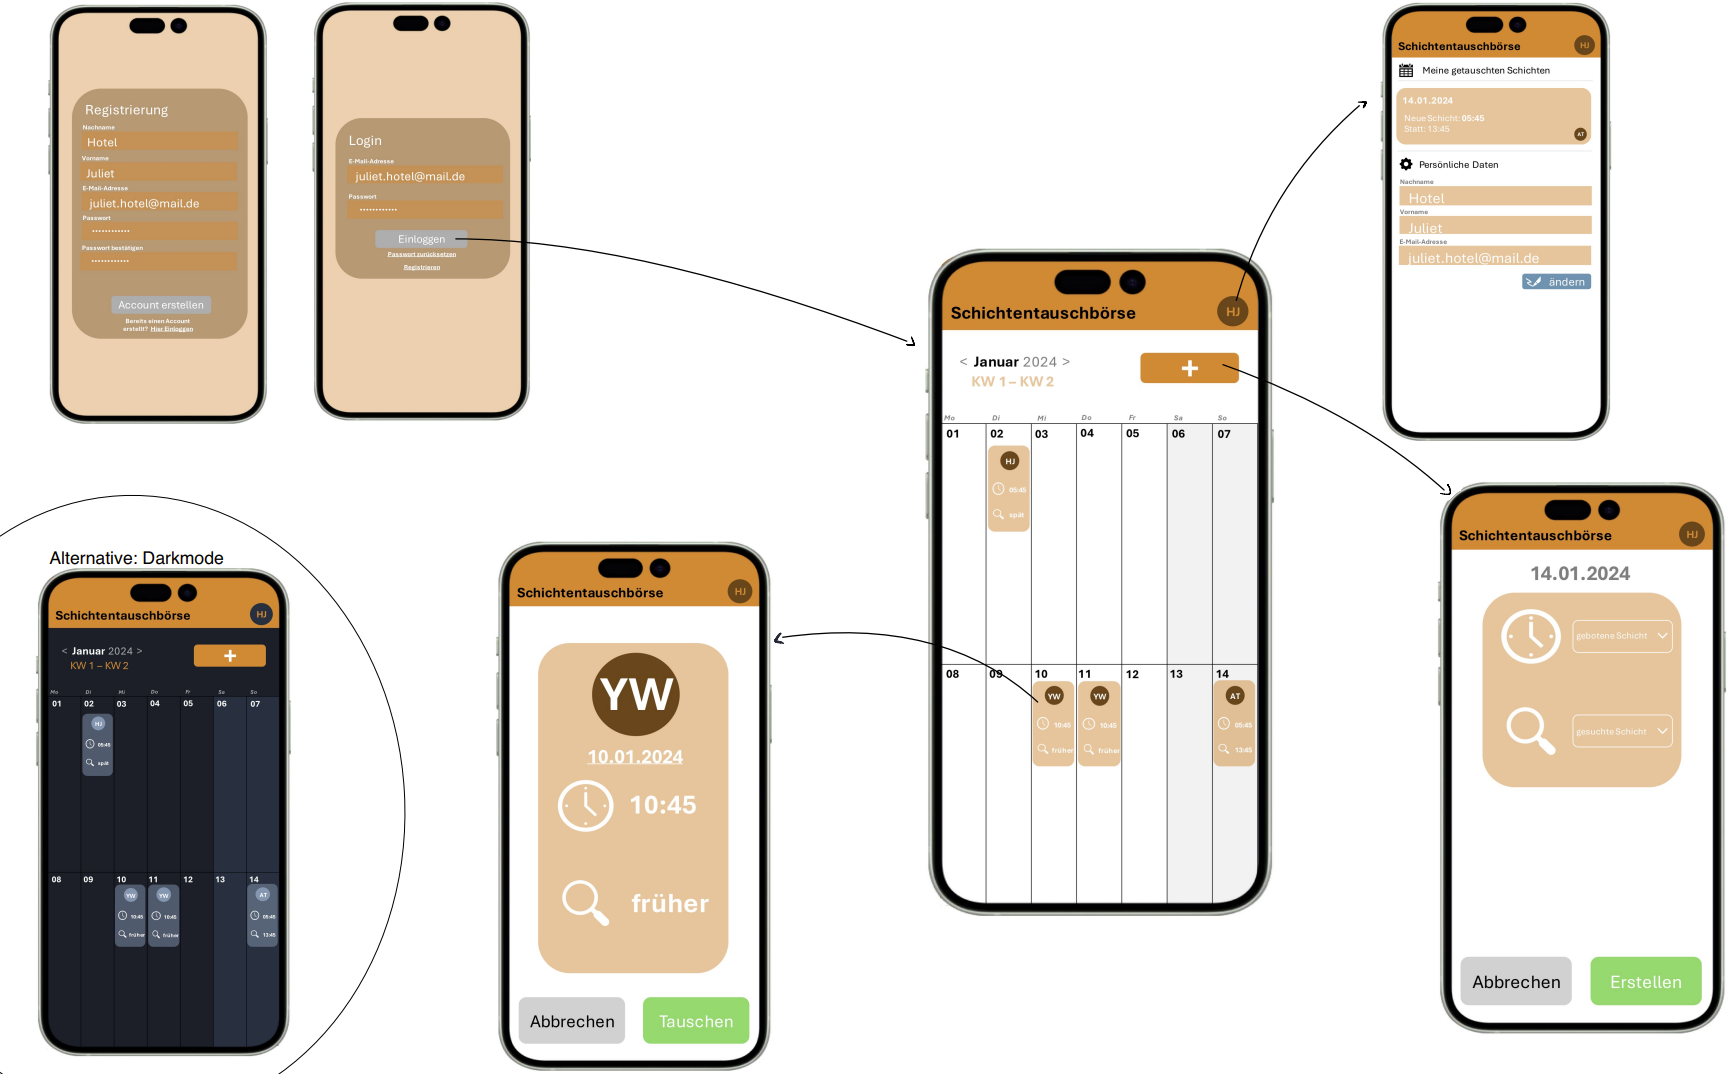
\includegraphics[clip,width=0.9\linewidth]{images/Bedienungskonzept_V1.png}
    \caption[Bedienungskonzept der Anwendung]{Bedienungskonzept der Anwendung}
    \label{Bedienungskonzept_V1}
\end{figure}

Nachdem sich der Nutzer registriert und anschließend erfolgreich angemeldet hat, gelangt er auf die zentrale Übersichtsseite, wie in Abbildung \ref{Bedienungskonzept_V1} dargestellt. 
Diese ermöglicht den Zugang zu allen anderen Seiten der Anwendung. 
Über die User-Kennung im Header gelangt der Nutzer zu einer Einstellungsseite. 
Dort kann er seine persönlichen Daten ändern und die bereits getauschten Schichten einsehen. 
Durch Klicken auf den Namen der Anwendung "Schichtentauschbörse" im Header gelangt er jederzeit zurück zur Übersicht.

Möchte ein Nutzer eine neue Tauschanfrage erstellen, ist das über den Button direkt unter dem Header möglich. 
Dabei wird eine neue Seite aufgerufen, auf der die gebotene und gesuchte Schicht aus einem Dropdown-Menü ausgewählt werden können. 
Alternativ kann der Nutzer auch eine bestimmte Uhrzeit eingeben, falls eine spezifische Zeit gewünscht ist. 
Wenn der Nutzer seine Anfrage doch nicht stellen möchte, kann er den Vorgang abbrechen und gelangt zurück zur Übersichtsseite. 
Mit dem Drücken des „Erstellen“-Buttons wird die neue Tauschanfrage finalisiert und im Kalender für alle Nutzer sichtbar.

Klickt ein Nutzer im Kalender auf eine Anfrage, kann er das Annehmen der Tauschanfrage entweder über den Button „Abbrechen“ beenden oder über den Button „Tauschen“ die Schicht tauschen. 
Nach dem Annehmen verschwindet die Tauschanfrage aus dem Kalender und wird in den Einstellungen unter „Meine getauschten Schichten“ angezeigt.

Zusätzlich wurde eine alternative Dark Mode-Version der Übersichtsseite erstellt, um unterschiedliche Präferenzen der Nutzer einzubinden.

\section{Phase 5: Nutzerumfrage}
\label{chap:nutzerumfrage}
\subsection{Methodik und Durchführung der Nutzerumfrage}

\subsection{Auswertung und Analyse der Nutzerumfrage}
\chapter{Fazit und Ausblick}

\backmatter
\sloppy
\printbibliography
\addcontentsline{toc}{chapter}{Literaturverzeichnis}

\end{document}